\section{Introducción}
	

El propósito de este capítulo es actualizar los coeficientes del indice CAPECO creado por el INDEC para utilizar en el marco del Censo 2001. Para ello utilizaremos los datos de la EPH correspondientes al tercer trimestre de 2010 de modo que coincida con el momento de relevamiento de datos del Censo 2010 (27 de octubre de 2010). Dado que nos concentramos en el Aglomerado Gran Buenos Aires, solamente tomaremos los datos pertenecientes a los aglomerados de Ciudad de Buenos Aires y Partidos del Gran Buenos Aires.  

Basándose en el paradigma del capital humano  \cite{mincer,beckar,schultz1961,schultz1962}, el modelo toma un conjunto de variables que puedan servir a aproximar el ingreso que perciben. Fundamentalmente, se considera el salario como una función de la productividad y la misma depende de factores como la experiencia y los años de escolaridad. Otras variables inciden en el mismo, pero no son relevadas en el Censo por lo cual quedan al margen del análisis. Al mismo tiempo, el género es un elemento a considerar dadas las iniquidades salariales empíricamente verificadas en diversos mercados laborales en el mundo y en la Argentina. 

Por lo tanto, se utilizan estos supuestos para construir un modelo que intente aproximarse al ingreso. Como se estableció previamente, el CAPECO intenta aproximar el Ingreso Per Cápita Familiar (IPCF). Sin embargo, al partir del modelo del capital humano se hace foco en los ingresos laborales. Si bien existen otras fuentes, éste continúa siendo el ingreso primordial de los hogares. A su vez los supuestos del capital humano para dar cuenta de los determinantes de este ingreso hace que el modelo resulte más preciso y legible. Incluir el ingreso total de las personas incluiría mayor fuente de variación que no sería explicada por el modelo. 

Por lo tanto, el modelo subyacente al CAPECO utiliza las siguientes variables para aproximarse al ingreso individual de las personas, previa transformación logarítmica de éste para establecer una relación \textit{log-lineal}, y utilizando al varón adulto de 35 años o más sin años de escolaridad como caso base o registro:

\begin{itemize}
	\item  Años de escolaridad primaria (\textit{aeprim})
	\item Años de escolaridad secundaria (\textit{aesec})
	\item Años de escolaridad universitaria (\textit{aeuniv})
	\item Varón entre 14 y 24 años (\textit{v14to24})
	\item Varón entre 25 y 34 años (\textit{v25to34})
	\item Mujer entre 14 y 24 años (\textit{m14to24})
	\item Mujer entre 25 y 34 años (\textit{m25to34})
	\item Mujer entre de 35 años o más (\textit{m35mas})
\end{itemize}

De esta manera el modelo queda especificado del siguiente modo:

$$Ln Y_n = Ln Y_0 + \beta_0 aeprim + \beta_1 aesec + \beta_2 aeuniv + $$
$$\beta_3 v14to24 + \beta_4 v25to34 +  \beta_5 m14to24 +  $$
$$\beta_6 m25to34 +  \beta_7 m35mas +  \cdots + \epsilon $$


El modelo original en base a datos de 2001 incluye la región a la que pertenece la persona (los ingresos varían según la región del país) y si la persona percibía jubilación o pensión. Sin embargo en este trabajo únicamente analizamos el modelo para la región del Aglomerado Gran Buenos Aires y en el censo 2010 no se preguntó en el formulario básico sobre la percepción de jubilación o pensión.

Este capítulo sigue la siguiente estructura. En primer lugar se pasa a hacer un análisis descriptivo de las variables utilizadas en el modelo. En segundo lugar, se implementa el modelo subyacente al CAPECO y se analizan sus resultados. En tercer lugar, se pasa a construir los coeficientes del índice CAPECO en base a la estimación de los parámetros del modelo. Finalmente se analiza la relación del CAPECO y el Ingreso Per Cápita Familiar.

\section{Exploración de las variables intervinientes}

En primer lugar analizamos la distribución del ingreso de la ocupación principal en escala logarítmica. 

\begin{figure}[!htb]
	\centering
	\textbf{Kernel density plot del Ingreso de la ocupación principal en escala logarítmica}\par\medskip
	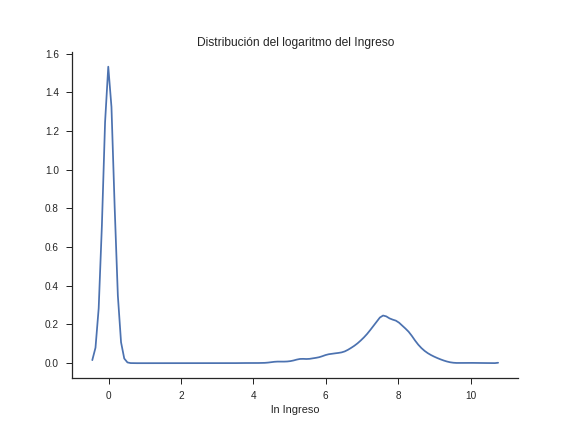
\includegraphics[scale = 0.5]{../img/capitulo3/kdePlotIngreso1.png}
	\caption{En la figura se puede observar cómo la distribución tiene dos picos: aquellos que no tienen ingresos y aquellos con ingresos.}
\end{figure}

Como se puede observar en el gráfico \ref{fig:kdePlotIngreso2} la mayoría de la población no percibe un ingreso profesional, lo cual es de esperar ya que su condición de actividad así lo indica (menores de 14 años, estudiantes, jubilados, desocupados, etc). 

\begin{figure}[!htb]
	\centering
	\textbf{Boxplot del ingreso de la ocupación principal según condición de actividad}\par\medskip
	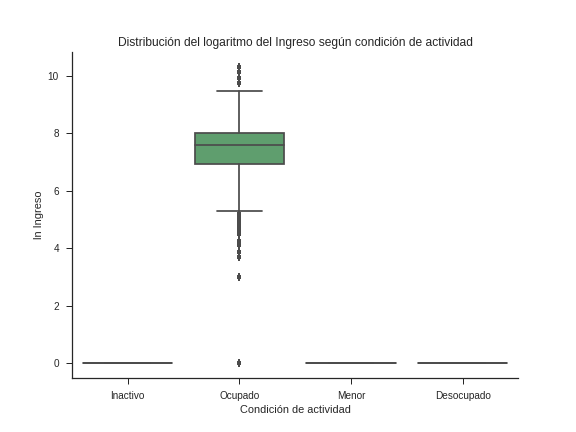
\includegraphics[scale = 0.5]{../img/capitulo3/kdePlotIngreso2.png}
	\caption{En la figura se puede observar la distribución para cada categoría de actividad. Como es de esperar, solo los ocupados registran ingresos de las ocupaciones principales.}
	\label{fig:kdePlotIngreso2}
\end{figure}

\begin{figure}[!htb]
	\centering
	\textbf{Boxplot de la proporción del ingreso salarial sobre el total según condición de actividad}\par\medskip
	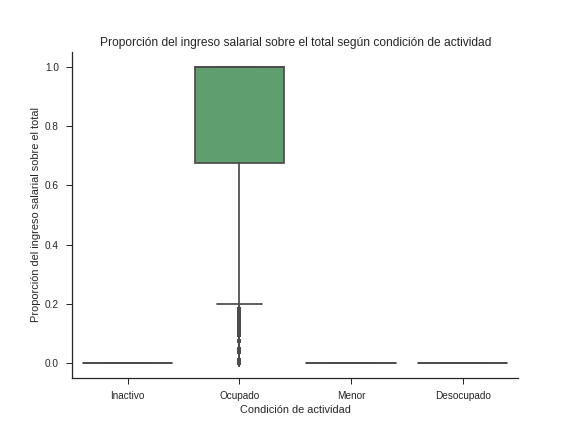
\includegraphics[scale = 0.5]{../img/capitulo3/ingresoSalarialVtotal.png}
	\caption{En la figura se puede observar que el grueso de los ingresos de los ocupados proviene de la ocupación principal.}
	\label{fig:ingresoSalarialVtotal}
\end{figure}

En ese sentido, procedemos a analizar únicamente a la población que tiene ingresos y una ocupación. Esto implica una limitación a la hora de percibir el conjunto de los ingresos (de los cuales los laborales, si bien una parte importante, constituyen solo una porción). Sin embargo, como se puede ver en el gráfico \ref{fig:ingresoSalarialVtotal} la mayoría de los ingresos provienen tienen como fuente la ocupación principal (para el 75\% de los casos los ingresos de lo ocupación principal explican \textit{al menos} el 67.5\% del ingreso total). Al mismo tiempo, las personas con trabajo que no perciben ingresos y tienen trabajo constituyen casos extremos o 
\textit{outliers} que pueden perjudicar la performance del modelo. Por ejemplo, esta situación puede deberse a que el trabajo es reciente y aún no cobraron el primer salario. Por lo tanto se decidió eliminar esos casos del análisis. 


Una vez eliminados esos casos, podemos observar la nueva distribución de la variable. Como se puede observar, no se aproxima a la distribución normal (el test de XXXXX arroja un p-valor de...). En el gráfico \ref{fig:kdePlotIngreso3} se puede observar la comparación de la distribución observada del ingreso con la distribución normal teórica.

\begin{figure}[!htb]
	\centering
	\textbf{Distribución del ingreso y la distribución normal}\par\medskip
	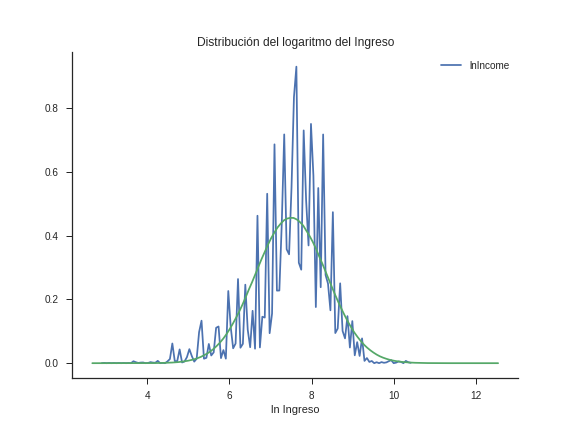
\includegraphics[scale = 0.5]{../img/capitulo3/kdePlotIngreso3.png}
	\caption{En la figura se puede observar que la distribución del ingreso en escala logarítmica no sigue la distribución normal.}
	\label{fig:kdePlotIngreso3}
\end{figure}

La brecha de ingresos en términos de género es un factor que incorpora en el análisis del CAPECO original. En base a datos de la EPH de 2010 se puede constatar que dicha brecha persiste. En términos de género se observa un ingreso menor por parte de las mujeres. La media del ingreso de la mujer es el 93.84 \% de la del varón (en escala logarítmica) mientras que la mediana, como se observa en el gráfico \ref{fig:ingresoVgenero}, representa el 95.31 \% de la del varón. En términos de ingreso, dicha diferencia se amplía a 70.55\% para la media y 69.57\% para la mediana. 


\begin{figure}[!htb]
	\textbf{Ingreso de la ocupación principal según género}\par\medskip
	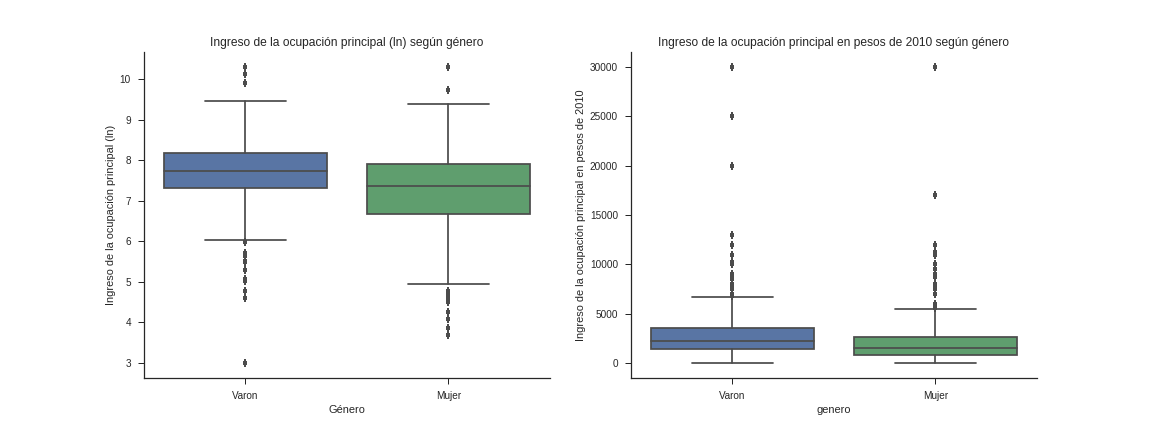
\includegraphics[scale = 0.4]{../img/capitulo3/ingresoVgenero.png}
	\caption{En la figura se puede observar que los varones tienen un ingreso superior en promedio al de las mujeres.}
	\label{fig:ingresoVgenero}
\end{figure}

Las otras variables presentes en el CAPECO son la edad y los años de escolaridad. Por lo tanto es necesario explorar las relaciones existentes entre la edad y el ingreso como así también entre éste y los años de escolaridad. Como se puede observar en el gráfico \ref{fig:ingresoVedadVescolaridad} existe una relación no lineal entre estas variables. En lo que corresponde a la edad, parece haber una relación creciente hasta pasados los 30 años. Llegada esa edad hay un amesetamiento por el cual no hay incrementos salariales a partir de la edad, para luego comenzar un proceso descendente (el año que inicia el cambio de tendencia hacia el descenso cambia de acuerdo al género: en las mujeres este proceso parece ser durante los 50s mientras que en los hombres en los 60s, lo que coincide con las diferencias en las edades jubilatorias legales). El comportamiento de la variable es similar (a pesar de una media de ingreso superior en los hombres). A mayor escolarización mayor salario. Pero esta relación no es lineal, sino que cada año de escolaridad de los tramos superiores ofrece mayores retornos que cada año de los tramos inferiores de escolaridad. Así por ejemplo un año adicional de universidad incrementa más el salario que un año adicional de primaria. En el anexo se puede ver el mismo esquema de análisis para separado por género en los gráficos \ref{fig:ingresoVedadVescolaridadMujeres} y \ref{fig:ingresoVedadVescolaridadVarones}

\begin{figure}[!htb]
	\textbf{Ingreso (ln) según género y escolaridad}\par\medskip
	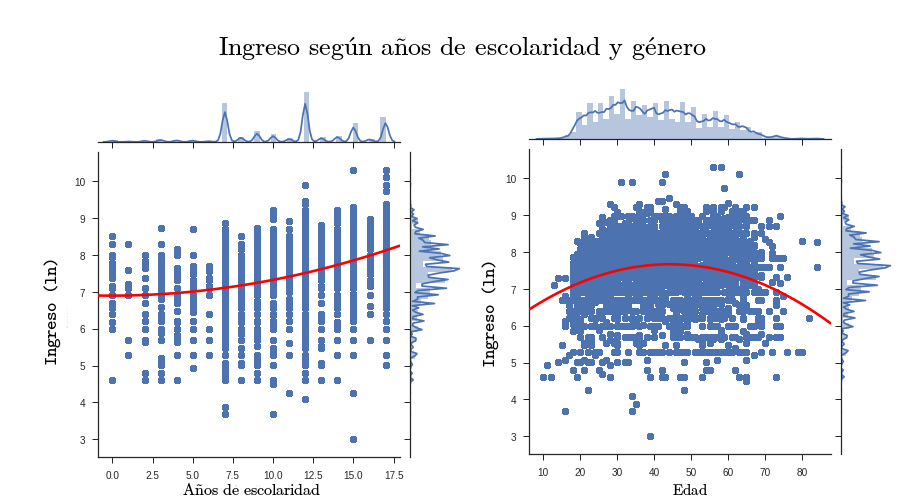
\includegraphics[scale = 0.4]{../img/capitulo3/ingresoVedadVescolaridad.png}
	\caption{.}
	\label{fig:ingresoVedadVescolaridad}
\end{figure}


Finalmente se puede ver en el gráfico \ref{fig:coormatrix} la matriz de correlación entre las variables que serán utilizadas en el modelo. En primer lugar el ingreso registra una correlación positiva con los años de escolaridad (0.40) y levemente negativa con el género en detrimento de las mujeres (-0.27). En términos de edad la correlación pareciera ser nula, pero como se observó en el gráfico \ref{fig:ingresoVedadVescolaridad} al ser una relación no lineal, el coeficiente de correlación puede ser engañoso. Se asume como evidente que no existe una correlación significativa entre edad y género, pero existen dos relaciones interesantes que surgen del análisis de esta matriz. En primer lugar, existe una muy leve correlación positiva entre género y escolaridad: lo que indicaría mayores años de escolaridad en promedio para las mujeres (0.13). En segundo lugar, una leve correlación negativa entre edad y años de escolaridad (-0.11). Las magnitudes de estas correlaciones son muy bajas pero merecen un mayor escrutinio. 


 
  \begin{figure}[!htb]
  	\centering
  	\textbf{Matriz de correlación - Variables seleccionadas}\par\medskip
  	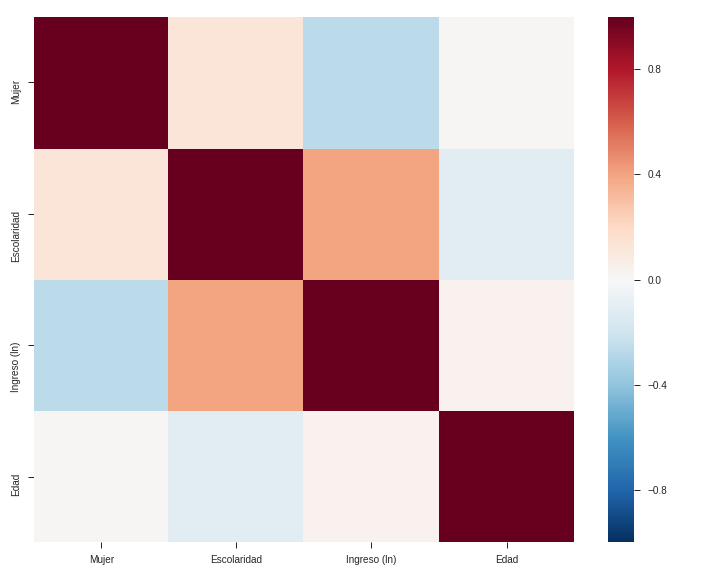
\includegraphics[scale = 0.4]{../img/capitulo3/corrMatrix.png}
  	\caption{.}
  	\label{fig:coormatrix}
  \end{figure}
  
Por un lado, en el gráfico \ref{fig:educVage} se puede ver que hay una leve tendencia a que, dentro de las personas con un trabajo, las más jóvenes tengan más años de escolaridad que las mayores. Una interpretación posible de esta situación es que el nuevo mundo del trabajo demanda más calificaciones por parte de sus recursos humanos a medida que los procesos se vuelven cada vez más tecnificados y especializados. Por otro lado, el gráfico \ref{fig:educVgenero} muestra una distribución de los años de escolaridad en las mujeres ligeramente asimétrica hacia los valores más altos de la variable. Dicho de otro modo, mientras que mujeres y varones presentan la misma mediana para años de escolaridad (10 años), la media de las mujeres es levemente superior (11.8 contra 10.8 años).
  
    \begin{figure}[!htb]
    	\centering
    	\textbf{Años de escolaridad según edad}\par\medskip
    	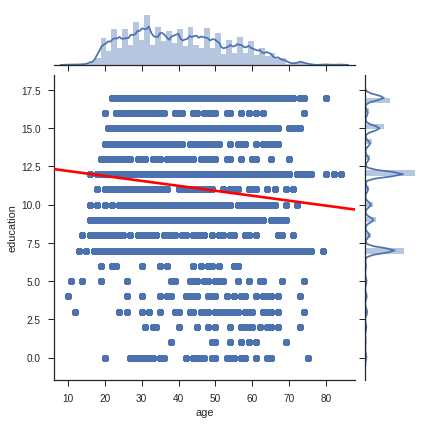
\includegraphics[scale = 0.4]{../img/capitulo3/educVage.png}
    	\caption{.}
    	\label{fig:educVage}
    \end{figure}

    \begin{figure}[!htb]
    	\centering
    	\textbf{Años de escolaridad según género}\par\medskip
    	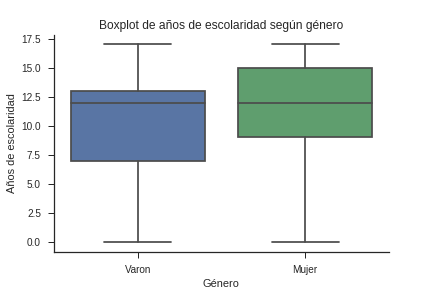
\includegraphics[scale = 0.4]{../img/capitulo3/educVgenero.png}
    	\caption{.}
    	\label{fig:educVgenero}
    \end{figure}
    
     
\section{El modelo y sus resultados}
A continuación procedemos a correr el modelo para todos los individuos con ingresos y que se encuentren empleados. La performance del mismo es disímil. Como se puede observar en la tabla \ref{tab:modelo} Si bien por un lado todos los parámetros son estadísticamente significativos para cualquier nivel de confianza, el modelo en su conjunto alcanza un $R^2$ de solo 27\%. Esto quiere decir que este modelo solo puede dar cuenta del 27\% de la variabilidad del logaritmo del ingreso. De todos modos es importante recordar que este modelo no considera elementos fundamentales para el ingreso como la cantidad de horas trabajadas o la rama en la que se desempeña cada persona. Diferentes ramas tienen diferentes productividades y por lo tanto pagan diferentes salarios.
    
    \begin{table}
    	\begin{tabular}{lrlr}
    		\textbf{Dep. Variable:}    &        y         & \textbf{  R-squared:         } &     0.274   \\
    		\textbf{Model:}            &       WLS        & \textbf{  Adj. R-squared:    } &     0.272   \\
    		\textbf{Method:}           &  Least Squares   & \textbf{  F-statistic:       } &     169.6   \\
    		\textbf{Date:}             & Sat, 15 Jul 2017 & \textbf{  Prob (F-statistic):} & 1.71e-243   \\
    		\textbf{Time:}             &     20:17:33     & \textbf{  Log-Likelihood:    } &   -4124.3   \\
    		\textbf{No. Observations:} &        3608      & \textbf{  AIC:               } &     8267.   \\
    		\textbf{Df Residuals:}     &        3599      & \textbf{  BIC:               } &     8322.   \\
    		\textbf{Df Model:}         &           8      & \textbf{                     } &             \\
    		
    	\end{tabular}
    	\begin{tabular}{lccccc}
    		& \textbf{coef} & \textbf{std err} & \textbf{t} & \textbf{P$>$$|$t$|$} & \textbf{[95.0\% Conf. Int.]}  \\
    		
    		\textbf{const} &       6.8690  &        0.093     &    73.616  &         0.000        &         6.686     7.052       \\
    		\textbf{aeprim}    &       0.0787  &        0.014     &     5.585  &         0.000        &         0.051     0.106       \\
    		\textbf{aesec}    &       0.0838  &        0.007     &    12.030  &         0.000        &         0.070     0.098       \\
    		\textbf{aeuniv}    &       0.1221  &        0.008     &    15.897  &         0.000        &         0.107     0.137       \\
    		\textbf{v14to24}    &      -0.4212  &        0.050     &    -8.364  &         0.000        &        -0.520    -0.322       \\
    		\textbf{v25to34}    &      -0.1547  &        0.039     &    -4.004  &         0.000        &        -0.230    -0.079       \\
    		\textbf{m14to24}    &      -0.9296  &        0.058     &   -15.926  &         0.000        &        -1.044    -0.815       \\
    		\textbf{m25to34}    &      -0.6264  &        0.043     &   -14.521  &         0.000        &        -0.711    -0.542       \\
    		\textbf{m35mas}    &      -0.5843  &        0.032     &   -17.988  &         0.000        &        -0.648    -0.521       \\

    	\end{tabular}
    	\begin{tabular}{lclc}
    		\textbf{Omnibus:}       & 667.857 & \textbf{  Durbin-Watson:     } &    1.855  \\
    		\textbf{Prob(Omnibus):} &   0.000 & \textbf{  Jarque-Bera (JB):  } & 1520.071  \\
    		\textbf{Skew:}          &  -1.050 & \textbf{  Prob(JB):          } &     0.00  \\
    		\textbf{Kurtosis:}      &   5.387 & \textbf{  Cond. No.          } &     60.5  \\
    		
    	\end{tabular}
    	\caption{Python Statsmodel WLS Regression Results}
    	\label{tab:modelo}
    \end{table}

De todos modos, el objetivo último de este modelo es ofrecer fundamento para los coeficientes del CAPECO. En todo caso veremos al final que capacidad tiene el CAPECO para dar cuenta de la variabilidad del ingreso.

En primer lugar, el intercepto da cuenta del ingreso esperado para un hombre adulto de 35 años o más con 0 años de escolaridad en cualquiera de los 3 niveles. Este constituye el caso base o registro con el cual compararemos al resto de los casos.

En segundo lugar los coeficientes dan cuenta de una relación Log-Nivel, esto quiere decir, por tomar el ejemplo del primer coeficiente (años de escolaridad primaria), que un año de escolaridad primaria ofrece un incremento de 7.87\% en el ingreso. Dicho de otro modo, un hombre adulto de 35 años o más con 1 año de escolaridad, gana un 7.87\% más que nuestro caso base (un hombre adulto de 35 años o más con 0 años de escolaridad). Del mismo modo, un año de escolaridad secundaria ofrece un incremento de 8.38\% y un año de escolaridad superior ofrece 12.21\%. Como es de esperar, los rendimientos no son lineales. Esto quiere decir que en el mercado laboral se valorizan más los años de escolaridad secundaria que los de primaria y los de educación superior a los de secundaria. El supuesto subyacente es que la productividad del trabajo aumenta con la capacitación que ofrece el sistema educativo.

En tercer lugar, los parámetros vinculados a la edad para los hombres, actúan como penalidades. Es decir, se supone que la edad conlleva experiencia y con ella mayor productividad. A su vez, el ciclo vital conlleva que los gastos de personas de tramos etarios superiores sean mayores. Es por ello que los hombres entre 14 y 24 años de edad sin años de escolaridad, ganarán un 42.12\% menos que el caso base, manteniendo todas las otras variables consideradas en el modelo constantes. A su vez, un hombre entre 25 y 34 años sin años de escolaridad tendrá un ingreso 15.47\% menor al del caso registro.

Finalmente, es necesario tomar en consideración el efecto del género conjugado con la edad. En primer lugar, parámetro que da cuenta del efecto del género al comparar una mujer de 35 años o más sin años de escolaridad con nuestro caso base (un hombre de idénticas características), nos dice que dicha mujer tendría un ingreso 58.43\% menor. Para los otros tramos de edades, una mujer entre 14 y 24 años dicha diferencia es de un 92.96\% menos y entre 25 y 34 años es de 62.64\% menos. 

\subsection{Análisis de resultados del modelo}

En términos de evaluación del modelo, los resultados también presentan una doble mirada. Por un lado se observa en el gráfico \ref{fig:predictedIncomeVincome.png} una relación lineal entre el ingreso observado y aquel estimado por el modelo. 

    \begin{figure}[!htb]
    	\centering
    	\textbf{Scatter plot y línea de regresión del ingreso observado y el estimado}\par\medskip
    	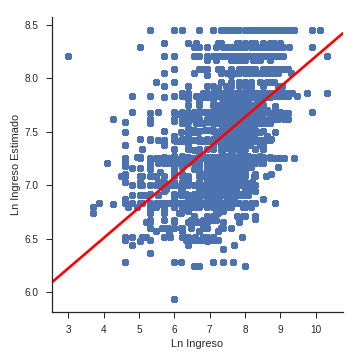
\includegraphics[scale = 0.4]{../img/capitulo3/predictedIncomeVincome.png}
    	\caption{.}
    	\label{fig:predictedIncomeVincome.png}
    \end{figure}

A su vez, al comparar los residuos en la escala original como en distancias con respecto a la media, se observa que los residuos se mueven mayoritariamente dentro de una franja aceptable. Al mismo tiempo, la media de los residuos es de 0.001. Sin embargo, como se puede observar en el gráfico \ref{fig:residuosNormales.png}, los mismos no se encuentran distribuidos normalmente.

    \begin{figure}[!htb]
    	\centering
    	\textbf{QQ plot de los residuos del modelo}\par\medskip
    	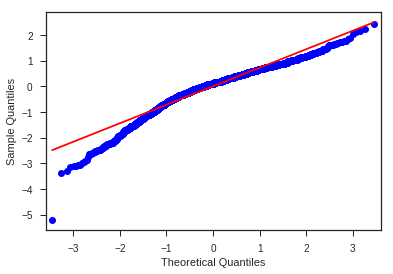
\includegraphics[scale = 0.4]{../img/capitulo3/residuosNormales.png}
    	\caption{El gráfico muestra que los residuos no se encuentran distribuidos normalmente}
    	\label{fig:residuosNormales.png}
    \end{figure}

Al hacer la comparación con los residuos estandarizados, se observa en el gráfico \ref{fig:residuosVestimado.png} que se mueven dentro de la franja de los 2 desvíos estándar, aunque con algunos casos moviéndose entre los 2 y 3 desvíos estándar por debajo de la media. Esto indica que este modelo peca de una ligera sobreestimación de los ingresos laborales en función de la edad, los años de escolaridad y el género. Esto no quiere decir que el CAPECO sobreestime los ingresos. Recordemos que este modelo se construye como fundamento de los coeficientes que utilizará el índice CAPECO. Una vez construido dicho índice, se puede analizar su desempeño como predictor del ingreso (en este caso será a su vez otro tipo de ingreso, el Ingreso Per Cápita Familiar).

    \begin{figure}[!htb]
    	\centering
    	\textbf{Scatter plot de residuos estandarizados según ingreso estimado}\par\medskip
    	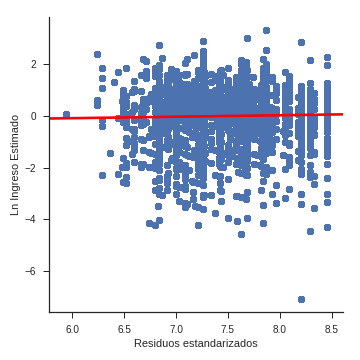
\includegraphics[scale = 0.4]{../img/capitulo3/residuosVestimado.png}
    	\caption{El gráfico muestra que los residuos se encuentran entre las franjas de los 2 desvíos estándar, con algunos casos por debajo (entre 3 y 4 desvíos estándar en relación a la media)}
    	\label{fig:residuosVestimado.png}
    \end{figure}

\section{Construcción del CAPECO y sus coeficientes}

$$\hat{Ln Y_n} = 6.87 + 0.078 * aeprim + 0.084 * aesec + 0.122 * aeuniv $$
$$ - 0.421 * v14to24 - 0.155 * v25to34 - 0.929 * m14to24  $$
$$-0.0626 * m25to34 - 0.584 * m35mas $$

VEMOS COMO LAS MUJERES NECESITAN MAS EDUCACION PARA COMPENSAR Y DE L AMISMA MANERA LOS MAS JOVENES TIENEN MAS EDUCACION POR ESO SE ACHICO LA BRECHA CON RESPECTO A 2001

A partir de estos parámetros del modelo, es necesario recontruir los coeficientes del CAPECO en base al modelo con datos actualizados con la EPH del tercer trimestre de 2010. Estos son:

$$ CAPECO = \frac{\displaystyle\sum_{i=1}^{n}(CP_i * VAE_i)}{\displaystyle\sum_{i=1}^{n}Aeq_i} $$

\begin{itemize}
	\item n: total de integrantes del hogar
	\item CP: condición de percepción (asume distintos valores según la condición de actividad, la edad, el sexo y el lugar de residencia)
	\item VAE: valor de los años de escolaridad invertidos en el mercado laboral
	\item Aeq: valor en unidades de adulto equivalente de cada integrante del hogar (varía de acuerdo al sexo y la edad, siguiendo una tabla de necesidades calóricas y nutricionales)
\end{itemize}

La metodología utilizada en el índice CAPECO original fue partir de un caso base y establecer comparaciones contra dicho valor base, a partir de incrementos en una unidad en la variable de interés. Esto quedará más claro en los ejemplos a continuación para cada coeficiente.

\subsection{Condición de Percepción CP - Genero y edad}

El coeficiente de \textbf{Condición de Percepción (CP)} intenta dar cuenta de los diferenciales en el ingreso en base a la edad y el género que se vienen describiendo en este capítulo. 

Para construir el CP se considera a los inactivos como coeficiente 0 y el caso base o registro (hombre de 35 años o más sin educación) como 1. A partir de esto se establece las proporciones contra el caso registro en base a género y edad. Esto quiere decir que se evalúa el valor que predice el modelo subyacente al CAPECO para el caso base y luego se compara contra el valor predicho por el modelo para otro caso donde se modifique una variable en una unidad. Es decir, se compara un hombre de 35 años o más sin educación contra un hombre entre 25 y 34 años sin educación para obtener el coeficiente para ese grupo etario. 

En términos de la ecuación del modelo, las variables que intervienen en el CP son de tipo \textit{dummy}, es decir toman valor 0 si se cumple una condición lógica (varón de 35 años o más) o si no la cumple:


\textbf{Caso registro}

$$962 = \exp (6.87 + 0.078 * 0 + 0.084 * 0 + 0.122 * 0 $$
$$ - 0.421 * 0 - 0.155 * 0 - 0.929 * 0  $$
$$-0.0626 * 0 - 0.584 * 0) $$

\textbf{Hombre entre 25 y 34 años sin educación}

$$824 = \exp (6.87 + 0.078 * 0 + 0.084 * 0 + 0.122 * 0 $$
$$ - 0.421 * 0 - 0.155 * 1 - 0.929 * 0  $$
$$-0.0626 * 0 - 0.584 * 0) $$

De este modo, el modelo predice que el caso base tiene ingresos laborales por \$962, mientras que un caso idéntico solo que de menor edad (entre 25 y 34 años) tiene ingresos por \$824. La relación entre ambos es de 0.8566, por lo que este será el coeficiente de CP para este último grupo. 	Si continuamos con este procedimiento, llegamos a la siguiente tabla de coeficientes para la Condición de Percepción en base a datos de 2010:






\begin{table}[h!]
	\centering
	\caption{Coeficientes de Percepción (CP) - 2010}
	\label{tab:tableCP}
	\begin{tabular}{l|c}
		Edad y género & CP \\
		\hline
		\hline
		Varón de 35 años o mas & 1 \\
		\hline
		Varón de 25 a 34 años & 0.86 \\
		\hline
		Varón de 14 a 24  años & 0.65 \\
		\hline
		Mujer de 35 años o mas & 0.56 \\
		\hline
		Mujer de 25 a 34 años & 0.53 \\
		\hline
		Mujer de 14 a 24  años & 0.39 \\
		
	\end{tabular}
\end{table}



Como se puede observar, se registran las mismas "penalidades" que en el modelo subyacente y que se encontraban en el CAPECO en base a datos de 2001.

Obviamente el caso registro siempre vale 1, sin importar el año. En lo que refiere a las penalidades por juventud mientras que para el tramo de hombres entre 25 y 34 años no cambió mucho de 2001 a 2010 (0.83 contra 0.86), el tramo de 14 a 24 disminuyó dichas penalidades (de 0.46 a 0.65). Mayores estudios sobre el mercado de trabajo son necesarios, aunque es posible arriesgar una hipótesis. El mercado dinámico de las nuevas tecnologías que creció enormemente en esa década, donde se puede presumir mejor adaptación por parte de los jóvenes en general, puede haber actuado como contrapeso a la falta de experiencia.

La situación de la mujer es paradógica. Comparar a la mujer de 35 años o más sin educación (lo que nos daría el efecto aislado del género más allá del efecto de la edad) muestra que la situación de la mujer empeoró levemente de 2001 a 2010 (pasa de tener un coeficiente de 0.60 a 0.56). Lo mismo sucede con el tramo de edad de 25 a 34 años (de 0.54 a 0.53). Sin embargo, al igual que con los hombres, existe una mejora para el tramo de 14 a 24 con respecto al 2001 (de 0.33 a 0.39).

\subsection{Valorización de los años de Escolaridad - VAE}

El coeficiente de \textbf{Valorización de los años de Escolaridad (VAE)} intenta dar cuenta de los retornos crecientes de los años de escolaridad en el ingreso por la ocupación principal.
 
En el trabajo del CAPECO de 2001, se decidió utilizar primaria completa como caso base de referencia. Esto quiere decir, que 7 años de escolaridad producían un valor de 7 para el coeficiente del VAE. Se mantuvo el mismo criterio en este trabajo con el fin de mantener la comparabilidad. Se evaluó el modelo para el caso base de un hombre de 35 años o más con 7 años de escolaridad primaria y se normalizó a 7. Luego se comparó este valor con los diferentes valores de años de escolaridad de los diferentes niveles.

\textbf{Hombre de 35 años o más con 7 años de escolaridad primaria}

$$1669 = \exp (6.87 + 0.078 * 7 + 0.084 * 0 + 0.122 * 0 $$
$$ - 0.421 * 0 - 0.155 * 0 - 0.929 * 0  $$
$$-0.0626 * 0 - 0.584 * 0) $$

\textbf{Hombre de 35 años o más con 6 años de escolaridad primaria}

$$1542 = \exp (6.87 + 0.078 * 1 + 0.084 * 0 + 0.122 * 0 $$
$$ - 0.421 * 0 - 0.155 * 0 - 0.929 * 0  $$
$$-0.0626 * 0 - 0.584 * 0) $$

\textbf{Cáculo del VAE para Hombre de 35 años o más con 6 años de escolaridad primaria}

$$\frac{1542}{1669}  * 7  = 6.47$$

La existencia de diversos sistemas educativos en diferentes provincias, así como las variaciones en los mismos hacia el interior de una provincia entre 2001 y 2010 hace realmente dificultoso el computar una variable como años de escolaridad. De todos modos se optó por una forma que intente compatibilizar los sistemas, aún sabiendo que puede haber dificultades en el cómputo. Por ejemplo una persona con séptimo grado de primaria completo en 2001 no es lo mismo que una persona con 7 de EGB, o 1 de la secundaria de la nueva Ley de Educación que convirtió esos niveles en secundaria. En todo caso, el código fuente de la función que realizó dichos cómputos contiene explícitamente las decisiones tomadas y se encuentra disponible en el repositorio para escrutinio de todo aquel que quiera explorar este problema.

Este procedimiento tiene por resultado la siguiente tabla de coeficientes \textbf{VAE}:

\begin{table}[h!]
	\centering
	\caption{Coeficientes de Percepción (CP) - 2010}
	\label{tab:tableCP}
	\begin{tabular}{l|c}
		Años aprobados & VAE \\
		\hline
		\hline
		0 & 4.0 \\
		1 & 4.4\\
		2 & 4.7 \\
		3 & 5.1 \\
		4 & 5.5 \\
		5 & 6.0 \\
		6 & 6.5 \\
		7 & 7.0 \\
		8 & 7.6 \\
		9 & 8.3 \\
		10 & 9.0  \\
		11 & 9.8 \\
		12 & 10.6 \\
		13 & 12.0 \\
		14 & 13.6 \\
		15 & 15.4\\
		16 & 17.3 \\
		17 &  19.6\\		
	\end{tabular}
\end{table}



El rango para la primaria no sufrió modificaciones. Varía entre 7 y 4. Para la secundaria, mientras que en 2001 variaba entre 7 y 11,1, en 2010 varía entre 7 y 10,6. Finalmente para la universidad, el valor máximo que registraba en 2001 era de 21.2 y en 2010 es de 19.6.

Se podría esgrimirse como posible hipótesis que el mercado laboral no valoriza tanto los estudios universitarios como antes o que en todo caso se han vuelto un nuevo estándar para un mercado laboral cada vez más tecnificado. Quizás si se extendiese el análisis de los años de escolaridad hacia los postgrados, se observaría alguna variación positiva.

\subsection{Adulto Equivalente}

Para la variación del Adulto Equivalente se procedió a tomar la nueva tabla provista por INDEC (\cite{indec2016b}) en base a la Encuestas de Gastos de los Hogares (ENGHO) más reciente (2004/5). El adulto equivalente se establece en base a determinar el requerimiento energético y las recomendaciones de nutrientes para las diferentes unidades de consumo o grupos etarios de los miembros de un hogar.aq


\begin{table}[!htbp]
	\centering
	\caption{Tabla de equivalencias de unidades consumidoras de adulto equivalente según edad y sexo}
	\label{tab:tableAE2004}
	\begin{tabular}{l|c|c}
		Sexo & Edad & Unidades consumidoras\\
		\hline
		\hline
		{} & 6 - 9 meses & 0,28 \\
		{} & 9 - 12 meses & 0,35 \\
		{} & 1 año & 0,37 \\
		{} & 2 años & 0,46 \\
		{} & 3 años & 0,51 \\
		Ambos & 4 años & 0,55 \\
		{} & 5 años & 0,60 \\
		{} & 6 años & 0,64 \\
		{} & 7 años & 0,66 \\
		{} & 8 años & 0,68 \\
		{} & 9 años & 0,69 \\
		\hline
		{} & 10 años & 0,79 \\
		{} & 11 años & 0,82 \\
		{} & 12 años & 0,85 \\
		Varones & 13 años & 0,90 \\
		{} & 14 años & 0,96 \\
		{} & 15 años & 1,00 \\
		{} & 16 años & 1,03 \\
		{} & 17 años & 1,04 \\
		\hline
		{} & 10 años & 0,70 \\
		{} & 11 años & 0,72 \\
		{} & 12 años & 0,74 \\
		Mujeres & 13 años & 0,76 \\
		{} & 14 años & 0,76 \\
		{} & 15 años & 0,77 \\
		{} & 16 años & 0,77 \\
		{} & 17 años & 0,77 \\
		\hline
		{} & 18-29 años & 1,02 \\
		{} & 30-45 años & 1,00 \\
		Varones & 46-60 años & 1,00 \\
		{} & 61-75 años & 0,83 \\
		{} & Más de 75 años & 0,74 \\
		\hline
		{} & 18-29 años & 0,76 \\
		{} & 30-45 años & 0,77 \\
		Mujeres & 46-60 años & 0,76 \\
		{} & 61-75 años & 0,67 \\
		{} & Más de 75 años & 0,63 \\
	\end{tabular}
\end{table}



\section{El CAPECO como predictor del Ingreso Per Capita Familiar}

Hasta ahora se utilizó el modelo del capital humano que intenta explicar el ingreso profesional a partir de la edad, el género y los años de escolaridad de las personas. En base a a los parámetros de dicho modelo, se construyeron los coeficientes del índice CAPECO. El mismo, consolidará para cada hogar el conjunto de las capacidades económicas de cada miembro activo del mismo para valorizar sus capitales en el mercado laboral. Una vez computado el índice CAPECO para todos los hogares, permitirá aproximarse a la capacidad económica de los mismos. Se testeará esta afirmación a partir de una regresión lineal entre el CAPECO y el Ingreso Per Cápita Familiar (IPCF). Con esto se busca observar qué capacidad tiene el CAPECO de dar cuenta de dicho ingreso.

\begin{table}
	\begin{tabular}{lrlr}
		\textbf{Dep. Variable:}    &        y         & \textbf{  R-squared:         } &     0.368   \\
		\textbf{Model:}            &       WLS        & \textbf{  Adj. R-squared:    } &     0.367   \\
		\textbf{Method:}           &  Least Squares   & \textbf{  F-statistic:       } &     1571.   \\
		\textbf{Date:}             & Sun, 16 Jul 2017 & \textbf{  Prob (F-statistic):} & 3.47e-271   \\
		\textbf{Time:}             &     11:14:23     & \textbf{  Log-Likelihood:    } &   -23422.   \\
		\textbf{No. Observations:} &        2703      & \textbf{  AIC:               } & 4.685e+04   \\
		\textbf{Df Residuals:}     &        2701      & \textbf{  BIC:               } & 4.686e+04   \\
		\textbf{Df Model:}         &           1      & \textbf{                     } &             \\
		
	\end{tabular}
	\begin{tabular}{lccccc}
		& \textbf{coef} & \textbf{std err} & \textbf{t} & \textbf{P$>$$|$t$|$} & \textbf{[95.0\% Conf. Int.]}  \\
		
		\textbf{const} &     640.9262  &       40.701     &    15.747  &         0.000        &       561.119   720.734       \\
		\textbf{CAPECO}    &     240.7351  &        6.074     &    39.633  &         0.000        &       228.825   252.645       \\
		
	\end{tabular}
	\begin{tabular}{lclc}
		\textbf{Omnibus:}       & 2099.363 & \textbf{  Durbin-Watson:     } &     1.896  \\
		\textbf{Prob(Omnibus):} &   0.000  & \textbf{  Jarque-Bera (JB):  } & 74203.272  \\
		\textbf{Skew:}          &   3.360  & \textbf{  Prob(JB):          } &      0.00  \\
		\textbf{Kurtosis:}      &  27.773  & \textbf{  Cond. No.          } &      10.4  \\
		
	\end{tabular}
	\caption{Python Stastmodels WLS Regression Results}
	\label{tab:capecoVipcf}
\end{table}  

Como se puede observar en la tabla \ref{tab:capecoVipcf} la performance no es buena. Si bien todos los estimadores de los parámetros son significativos para cualquier nivel de confianza, la $R^2$ es meramente un 0.368. Al observar el gráfico \ref{fig:capecoVipcf.png}, se puede observar la presencia de \textbf{outliers} o casos extremos que inciden en el comportamiento del modelo. Estos casos son aquellos hogares donde la totalidad de sus miembros son inactivos por diferentes motivos (estudiantes, jubilados, pensionados, amas de casa, rentistas, etc.) que perciben algún tipo de ingreso cuya fuente no es laboral. Esto puede ser becas, jubilaciones, pensiones, rentas, etc. La capacidad del CAPECO para inferir el ingreso de estos hogares es nula, como muestra la pendiente para esos casos. También se consideraron como \textit{outliers} los ingresos superiores a \$12000 (el 2\% de los casos). Al eliminar el análisis los mismos, el comportamiento del modelo mejora sustancialmente. 


     \begin{figure}[!htb]
     	\centering
     	\textbf{Scatter plot de IPCF según CAPECO y condición de actividad}\par\medskip
     	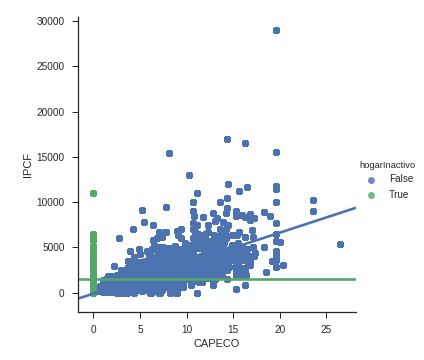
\includegraphics[scale = 0.4]{../img/capitulo3/capecoVipcf.png}
     	\caption{El gráfico muestra la relación existente entre el CAPECO y el IPCF para todos los hogares en azul y para aquellos cuya totalidad de los miembros son inactivos en verde. Como se puede ver, éstos últimos presentan un valor nulo en CAPECO pero disimiles IPCF}
     	\label{fig:capecoVipcf.png}
     \end{figure}
     
Como se puede apreciar en la tabla \ref{tab:capecoVipcfSinOut}, al eliminar los \textit{outliers} la $R^2$ del modelo aumenta a .506. A su vez, el estimador del parámetro CAPECO es significativo para cualquier nivel de confianza. El mismo indica que por cada punto de incremento del índice, el hogar recibe un incremento de \$296 en su Ingreso Per Cápita Familiar. El intercepto o parámetro constante es no significativo y en términos de magnitud puede asumir valores negativos, lo cual no tiene sentido ya que implicaría ingreso negativo de los hogares. Esto es una consecuencia de eliminar del análisis los hogares con CAPECO igual a 0.

\begin{table}
	\begin{tabular}{lrlr}
		
		\textbf{Dep. Variable:}    &        y         & \textbf{  R-squared:         } &     0.506   \\
		\textbf{Model:}            &       WLS        & \textbf{  Adj. R-squared:    } &     0.506   \\
		\textbf{Method:}           &  Least Squares   & \textbf{  F-statistic:       } &     2258.   \\
		\textbf{Date:}             & Sun, 16 Jul 2017 & \textbf{  Prob (F-statistic):} &     0.00    \\
		\textbf{Time:}             &     13:45:55     & \textbf{  Log-Likelihood:    } &   -18734.   \\
		\textbf{No. Observations:} &        2205      & \textbf{  AIC:               } & 3.747e+04   \\
		\textbf{Df Residuals:}     &        2203      & \textbf{  BIC:               } & 3.748e+04   \\
		\textbf{Df Model:}         &           1      & \textbf{                     } &             \\
		
	\end{tabular}
	\begin{tabular}{lccccc}
		& \textbf{coef} & \textbf{std err} & \textbf{t} & \textbf{P$>$$|$t$|$} & \textbf{[95.0\% Conf. Int.]}  \\
		
		\textbf{const} &      68.3721  &       46.201     &     1.480  &         0.139        &       -22.230   158.974       \\
		\textbf{CAPECO}    &     295.7912  &        6.225     &    47.517  &         0.000        &       283.584   307.999       \\
		
	\end{tabular}
	\begin{tabular}{lclc}
		\textbf{Omnibus:}       & 911.298 & \textbf{  Durbin-Watson:     } &    1.919  \\
		\textbf{Prob(Omnibus):} &   0.000 & \textbf{  Jarque-Bera (JB):  } & 6844.574  \\
		\textbf{Skew:}          &   1.768 & \textbf{  Prob(JB):          } &     0.00  \\
		\textbf{Kurtosis:}      &  10.874 & \textbf{  Cond. No.          } &     14.0  \\
		
	\end{tabular}
	\caption{Python Statsmodels WLS Regression Results}
	\label{tab:capecoVipcfSinOut}
\end{table}

En términos de análisis de resultados del modelo, se observa que hay una importante variación en los residuos, en especial hacia los valores positivos, lo que indica una \textit{subestimación} de ingresos por parte del CAPECO. Esto puede deberse a que a iguales condiciones en las variables observadas por el modelo, existen diferencias en las variables no observadas que causan un ingreso mayor (pueden ser más horas trabajadas o que los miembros activos del hogar se desempeñan en sectores de mayores productividades) 


     \begin{figure}[!htb]
     	\centering
     	\textbf{Scatter plot de ingreso estimado según ingreso observado}\par\medskip
     	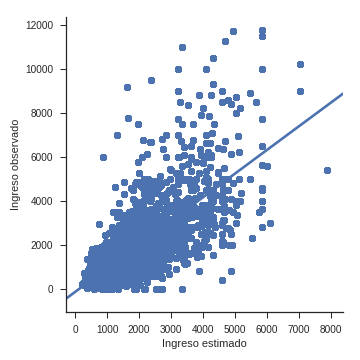
\includegraphics[scale = 0.4]{../img/capitulo3/evalCapecoVipcf1.png}
     	\caption{}
     	\label{fig:evalCapecoVipcf1.png}
     \end{figure}
     
     \begin{figure}[!htb]
     	\centering
     	\textbf{Scatter plot de residuos estandarizados según ingreso observado}\par\medskip
     	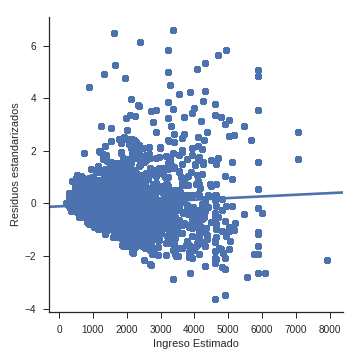
\includegraphics[scale = 0.4]{../img/capitulo3/evalCapecoVipcf2.png}
     	\caption{}
     	\label{fig:evalCapecoVipcf2.png}
     \end{figure}
     
     \begin{figure}[!htb]
     	\centering
     	\textbf{QQ plot de}\par\medskip
     	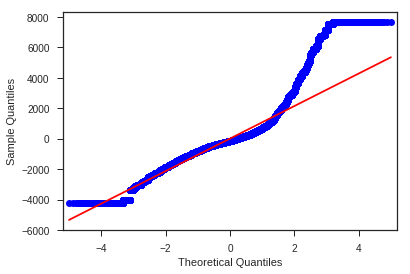
\includegraphics[scale = 0.4]{../img/capitulo3/evalCapecoVipcf3.png}
     	\caption{}
     	\label{fig:evalCapecoVipcf3.png}
     \end{figure}     
     
     \begin{table}[h!]
     	\centering
     	\caption{Condición de inactividad para los miembros de hogares con totalidad de miembros inactivos}
     	\label{tab:tableInactivos}
     	\begin{tabular}{l|c}
     		Condición de inactividad & \% \\
     		\hline
     		\hline
     		Jubilado - Pensionado &  86.3 \\
     		Ama de casa & 6.0\\
     		Estudiante &  5.1\\
     		Otros &   1.2\\
     		Discapacitado/a & 1.0 \\
     		Rentista &  0.4\\	
     	\end{tabular}
     \end{table}
          
     
Antes de concluir, es interesante analizar el comportamiento de los hogares que obtienen 0 en el CAPECO porque la totalidad de sus miembros son inactivos. Esta es la principal debilidad del índice, su incapacidad para inferir ingresos para está población. Al observar en más detalle cómo está caracterizada, se observa que el 86.3 \% son jubilados. Mientras que en 2001 el Censo preguntaba por la percepción de jubilación, el CAPECO original podía percibir dicho efecto en el ingreso. Lamentablemente el instrumento censal básico de 2010, el único que permite obtener resultados a nivel de radio censal, no realizó esa pregunta. Por lo tanto no se puede inferir el ingreso a partir de la misma, abriendo este flanco débil al índice.   